\newpage
\section{Hàm số liên tục}
\subsection{KIẾN THỨC CẦN NHỚ}
\subsubsection{Hàm số liên tục tại một điểm}
\begin{dn}
	Cho hàm số $y=f(x)$ xác định trên khoảng $K$ và $x_0\in K$.\\
	Hàm số $y=f(x)$ được gọi là liên tục tại điểm $x_0$ nếu $\lim\limits_{x\to x_0} f(x)=f\left(x_0\right)$.
\end{dn}
\begin{nx}
	Để hàm số $y=f(x)$ liên tục tại $x_0$ thì phải có cả ba điều sau
	\begin{enumerate}
		\item Hàm số xác định tại $x_0$.
		\item Tồn tại $\lim\limits_{x\to x_0}f(x)$.
		\item $\lim\limits_{x\to x_0}f(x)=f\left(x_0\right)$.
	\end{enumerate}
\end{nx}	
\begin{luuy}
	Khi hàm số $y=f(x)$ không liên tục tại điểm $x_0$ thì ta nói $f(x)$ gián đoạn tại điểm $x_0$ và $x_0$ được gọi là điểm gián đoạn của hàm số $f(x)$.
\end{luuy}
\subsubsection{Hàm số liên tục trên một khoảng, trên một đoạn}

\begin{dn}\hfill
	\begin{itemize}
		\item Cho hàm số $y=f(x)$ xác định trên khoảng $(a;b)$.\\
		Hàm số $y=f(x)$ được gọi là liên tục trên khoảng $(a;b)$ nếu $f(x)$ liên tục tại mọi điểm trong khoảng ấy.
		\item Cho hàm số $y=f(x)$ xác định trên đoạn $[a;b]$.\\
		Hàm số $y=f(x)$ được gọi là liên tục trên đoạn $[a;b]$ nếu $f(x)$ liên tục tại trên khoảng $(a;b)$ và $\lim\limits_{x\to a^+}f(x)=f(a)$, $\lim\limits_{x\to b^-}f(x)=f(b)$.
	\end{itemize}
	
\end{dn}
\begin{nx}
	\immini{Đồ thị của hàm số $y=f(x)$ liên tục trên đoạn $[a;b]$ là một đường liền, có điểm đầu, điểm cuối như hình vẽ bên. Nếu hai điểm này nằm về hai phía so với trục hoành thì đường liền nói trên luôn cắt trục hoành tại ít nhất một điểm. Điều này có thể được phát biểu dưới dạng như sau:\\
		Nếu hàm số $y=f(x)$ liên tục trên $[a;b]$ và $f(a)\cdot f(b)<0$ thì luôn tồn tại ít nhất một điểm $c\in(a;b)$ sao cho $f(c)=0$.
	}{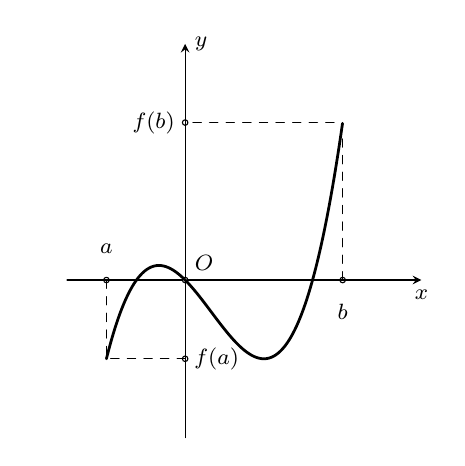
\begin{tikzpicture}[>=stealth,line join=round,line cap=round,font=\footnotesize,scale=1]
		\draw [->] (-1.5,0)--(3,0)node[below]{\footnotesize $x$};
		\draw [->] (0,-2)--(0,3)node[right]{\footnotesize $y$};
		\draw [fill=white,draw=black] (0,0) circle (1pt)node[above right] {\footnotesize $O$};
		\draw [dashed](-1,0)--(-1,-1)--(0,-1) (2,0)--(2,2)--(0,2);
		\clip(-2,-1.5) rectangle (3,3);
		\draw[line width=1.0pt,smooth,samples=100,domain=-1:2]  plot(\x,{(\x)^3-(\x)^2-(\x)});
		\draw (0,-1) node[shift={(0:.4)}]{$f(a)$} circle (1pt);
		\draw (0,2) node[shift={(180:.4)}]{$f(b)$} circle (1pt);
		\draw (-1,0) node[shift={(90:.4)}]{$a$} circle (1pt);
		\draw (2,0) node[shift={(-90:.4)}]{$b$} circle (1pt);
		\end{tikzpicture}}
\end{nx}
\subsubsection{Tính liên tục của hàm số sơ cấp}

\begin{dn}\hfill
	\begin{itemize}
		\item Hàm số đa thức $P(x)$, các hàm số lượng giác $y=\sin x$, $y=\cos x$ liên tục trên $\mathbb{R}$.
		\item Hàm số phân thức $y=\dfrac{P(x)}{Q(x)}$, hàm số căn thức $y=\sqrt{P(x)}$, các hàm số lượng giác $y=\tan x$, $y=\cot x$ liên tục trên các khoảng của tập xác định của chúng.\\
		Trong đó, $P(x)$ và $Q(x)$ là các đa thức.
	\end{itemize}
\end{dn}
\begin{nx}
	Hàm số thuộc những loại trên được gọi chung là hàm số sơ cấp. Khi nói xét tính liên tục của một hàm số mà không nói gì thêm thì ta xét tính liên tục của hàm số đó trên những khoảng của tập xác định của chúng.
\end{nx}		
\subsubsection{Tổng, hiệu, tích, thương của hàm số liên tục}

\begin{dn}
	Cho hai hàm số $y=f(x)$ và $y=g(x)$ liên tục tại điểm $x_0$. Khi đó:
	\begin{itemize}
		\item Các hàm số $y=f(x)+g(x)$, $y=f(x)-g(x)$, $y=f(x)\cdot g(x)$ liên tục tại $x_0$.
		\item Hàm số $y=\dfrac{f(x)}{g(x)}$ liên tục tại $x_0$ nếu $g\left(x_0\right)\ne0$.
	\end{itemize}
\end{dn}
\subsection{PHÂN LOẠI VÀ PHƯƠNG PHÁP GIẢI TOÁN}
\begin{dang}{Xét tính liên tục của hàm số tại một điểm}
		Cho hàm số $y=f(x)$ xác định trên tập $\mathscr{D}$. Để xét tính liên tục của hàm số $y=f(x)$ tại điểm $x_{0}\in \mathscr{D}$, ta thực hiện các bước sau:
	\begin{itemize}
		\item [\iconMT] Bước 1. Tính $f(x_0)$.
		\item [\iconMT] Bước 2. Tìm $\lim\limits_{x\to x_0}f(x)$.
		\item [\iconMT] Bước 3. So sánh và rút ra kết luận.
		\begin{itemize}
			\item Nếu $\lim\limits_{x\to x_0}f(x)=f(x_0)$ thì hàm số $f(x)$ liên tục tại điểm $x_0$.
			\item Nếu $\lim\limits_{x\to x_0}f(x)\ne f(x_0)$ thì hàm số $f(x)$ không liên tục (gián đoạn) tại điểm $x_0$.
		\end{itemize}
	\end{itemize}
\end{dang}
\begin{vd}[\itshape{SGK CTST 11}]%[Dự án đề cương 3 khối năm học 2024 - 2025]%[LamNguyen]%[1D3N3-3]
Xét tính liên tục của hàm số:
	\begin{enumerate}
		\item $f(x)=\heva{&x^2+1&\quad\text{khi }&x\ge0\\&1-x&\quad\text{khi }&x<0}$ tại điểm $x=0$.
		\item $f(x)=\heva{&x^2+2&\quad\text{khi }&x\ge1\\&x&\quad\text{khi }&x<1}$ tại điểm $x=1$.
	\end{enumerate}
	\loigiai{\begin{enumerate}
			\item Ta có $\heva{& f(0)=0^2+1=1\\
			&\lim\limits_{x\to0^+}f(x)=\lim\limits_{x\to0^+}\left(x^2+1\right)=0^2+1=1 \\&\lim\limits_{x\to0^-}f(x)=\lim\limits_{x\to0^-}(1-x)=1-0=1.}$\\
			Do $\lim\limits_{x\to0^-}f(x)=\lim\limits_{x\to 0^+}f(x)=f(0)$ nên hàm số $y=f(x)$ liên tục tại điểm $x=0$.
			\item Ta có
			$\heva{&f(1)=1^2+2=3 \\&\lim\limits_{x\to1^+}f(x)=\lim\limits_{x\to1^+}\left(x^2+2\right)=1^2+2=3 \\& \lim\limits_{x\to1^-}f(x)=\lim\limits_{x\to1^-}(x)=1=1 .}$\\
			Do $\lim\limits_{x\to1^+}f(x)\ne\lim\limits_{x\to1^-}f(x)$ nên không tồn tại $\lim\limits_{x\to1}f(x)$.\\
			Vậy hàm số $y=f(x)$ không liên tục tại điểm $x=1$.
	\end{enumerate}}
\end{vd}
\begin{vd}%[1D3H3-3]%[Dự án đề cương 3 khối năm học 2024 - 2025]%[LamNguyen]
	Xét tính liên tục của hàm số $f(x)=\heva{&\dfrac{x^2-3x+2}{x-2}&\text{khi }x\neq 2\\&4x-7&\text{khi }x=2}$ tại điểm $x_0=2$.
	\loigiai{
		Ta có $f(x_0)=f(2)=4\cdot 2-7=1$.\\
		$\lim\limits_{x\rightarrow2}f(x)=\lim\limits_{x\rightarrow2}\dfrac{x^2-3x+2}{x-2}=\lim\limits_{x\rightarrow2}\dfrac{(x-1)(x-2)}{x-2}=\lim\limits_{x\rightarrow2}(x-1)=1$.\\
		Vì $f(2)=\lim\limits_{x\rightarrow 2}f(x)$ nên hàm số $f(x)$ liên tục tại điểm $x_0=2$.
	}
\end{vd}
\begin{dang}{Xét tính liên tục của hàm số trên miền xác định}
	\begin{itemize}
		\item [\iconMT] Hàm đa thức liên tục trên $\mathbb{R}$.
		\item [\iconMT] Hàm phân thức hữu tỉ, hàm lượng giác liên tục trên từng khoảng xác định của chúng.
	\end{itemize}
\end{dang}
\begin{vd}[\itshape{SGK CTST 11}]%[1D3H3-4]%[Dự án đề cương 3 khối năm học 2024 - 2025]%[LamNguyen]
	Xét tính liên tục của các hàm số sau
	\begin{enumEX}{3}
		\item $f(x)=\dfrac{x}{x^2-4}$.
		\item $g(x)=\sqrt{9-x^2}$.
		\item $h(x)=\cos x+\tan x$.
	\end{enumEX}
	\loigiai{\begin{enumerate}
			\item Hàm số $f(x)=\dfrac{x}{x^2-4}$ là hàm phân thức, có tập xác định là $\mathscr{D}=(-\infty;-2)\cup(-2;2)\cup(2;+\infty)$ nên nó liên tục trên các khoảng $(-\infty;-2)$, $(-2;2)$, $(2;+\infty)$.
			\item Hàm số $g(x)=\sqrt{9-x^2}$ là hàm số có tập xác định là $\mathscr{D}=[-3;3]$ nên nó liên tục trên đoạn $[-3;3]$.
			\item Hàm số $y=\cos x$ liên tục tại mọi điểm $x_0\in\mathbb{R}$.\\
			Hàm số $y=\tan x$ liên tục tại mọi điểm $x_0\ne\dfrac{\pi}{2}+k\pi$, $k\in\mathbb{Z}$.\\
			Do đó nên hàm số $y=\cos x+\tan x$ liên tục tại mọi điểm $x_0\ne\dfrac{\pi}{2}+k\pi$, $k\in\mathbb{Z}$.
	\end{enumerate}}
\end{vd}
\begin{vd}%[1D3H3-4]%[Dự án đề cương 3 khối năm học 2024 - 2025]%[LamNguyen]
	Xét tính liên tục của hàm số sau trên tập xác định của chúng.
	\begin{tasks}(2)
		\task $f(x)=\heva{&\dfrac{x^2-x-2}{x+1}&\text{ khi } x\ne -1\\ &-3&\text{ khi } x=-1}$.
		\task $f(x)=\heva{&\dfrac{2x+1}{(x-1)^2}&\text{ khi } x\ne 1\\ &3 &\text{ khi } x=1}$.
	\end{tasks}
	\loigiai{
		\begin{enumerate}
			\item \begin{itemize}
				\item Tập xác định của hàm số là $\mathscr{D}=\mathbb{R}$.
				\item Khi $x \ne -1$, $f(x)=\dfrac{x^2-x-2}{x+1}$ là hàm phân thức hữu tỉ nên liên tục trên $(-\infty;-1)\cup(-1;+\infty)$.
				\item Tại điểm $x=-1$, ta có $f(-1)=-3$.\\
				$\lim\limits_{x\to -1}f(x)=\lim\limits_{x\to -1}\dfrac{x^2-x-2}{x+1}=\lim\limits_{x\to -1}(x-2)=-3=f(-1).$\\
				Do đó hàm số liên tục tại $x=-1$.
				\item Vậy hàm số liên tục trên $\mathbb{R}$.
			\end{itemize}
			\item \begin{itemize}
				\item Tập xác định của hàm số là $\mathscr{D}=\mathbb{R}$.\\
				\item Khi $x \ne 1$, $f(x)=\dfrac{2x+1}{(x-1)^2}$ là hàm phân thức hữu tỉ nên liên tục trên $(-\infty;1)\cup(1;+\infty)$.\\
				\item Tại điểm $x=1$, ta có $f(1)=3$.\\
				$\lim\limits_{x\to 1}f(x)=\lim\limits_{x\to 1}\dfrac{2x+1}{(x-1)^2}=+\infty\ne f(-1).$\\
				Do đó hàm số gián đoạn tại $x=1$.
				\item Vậy hàm số liên tục trên $\mathbb{R}\setminus\{1\}$.
			\end{itemize}
	\end{enumerate}}
\end{vd} 
\begin{dang}{Tìm giá trị tham số để hàm số liên tục}
Sử dụng định nghĩa: \\
Cho hàm số $y=f(x)$ xác định trên khoảng $K$ và $x_0\in K$.\\
Hàm số $y=f(x)$ được gọi là liên tục tại điểm $x_0$ nếu $\lim\limits_{x\to x_0} f(x)=f\left(x_0\right)$.\\
Từ đó giải phương trình tìm tham số.
\end{dang}
\begin{vd}[\itshape{SGK CTST 11}]%[1D3H3-3]%[Dự án đề cương 3 khối năm học 2024 - 2025]%[LamNguyen]
	Cho hàm số $f(x)=\heva{&\dfrac{x^2-4}{x+2}&\quad\text{khi }&x\ne-2\\&a&\quad\text{khi }&x=-2.}$\\
	Tìm $a$ để hàm số $y=f(x)$ liên tục trên $\mathbb{R}$.
	\loigiai{Với mọi $x_0\ne-2$, ta có $f(x)=\dfrac{x^2-4}{x+2}$ luôn xác định nên liên tục trên các khoảng $(-\infty;-2)$ và $(-2;+\infty)$.\\
		Mặt khác ta có $f(-2)=a$, $\lim\limits_{x\to-2}f(x)=\lim\limits_{x\to-2}\dfrac{x^2-4}{x+2}=\lim\limits_{x\to-2}(x-2)=-2-2=-4$.\\
		Để hàm số $y=f(x)$ liên tục trên $\mathbb{R}$ thì hàm số $y=f(x)$ phải liên tục tại $x=-2$
		$$\lim\limits_{x\to-2}f(x)=f(-2)\Leftrightarrow a=-4.$$}
\end{vd}
\begin{vd}%[1D3H3-3]%[Dự án đề cương 3 khối năm học 2024 - 2025]%[LamNguyen]
	Tìm tham số $ m $ để hàm số $ f(x) = \heva{&\dfrac{x^2 - 2x - 3}{x+1}   &\text{  khi }  x \neq -1\\&m^2 + 5m  &\text{  khi } x = -1} $liên tục tại $ x_0 = -1. $
	\loigiai{
		Ta có: $ \lim\limits_{x \to -1} f(x) =  \lim\limits_{x \to -1} \dfrac{x^2 - 2x - 3}{x+1}  = \lim\limits_{x \to -1} \dfrac{(x+1)(x-3)}{x+1} = \lim\limits_{x \to -1} (x-3)  = -4$.\\
		$ f(-1) = m^2 + 5m $.\\
		Hàm số liên tục tại $ x_0 = -1 \Leftrightarrow m^2 + 5m = -4 \Leftrightarrow \hoac{m=-1\\m=-4}. $
	}	
\end{vd} 
\begin{dang}{Chứng minh phương trình có nghiệm}
	\begin{itemize}
		\item Để chứng minh phương trình $f(x)=0$ có ít nhất một nghiệm trên $\mathscr{D}$, ta chứng minh hàm số $y=f(x)$ liên tục trên $ D $ và có hai số $a,b\in \mathscr{D}$ sao cho $f(a)\cdot f(b)<0$. 
		\item Để chứng minh phương trình $f(x)=0$ có $ k $ nghiệm trên $\mathscr{D}$, ta chứng minh hàm số $y=f(x)$ liên tục trên $D$ và tồn tại $k$ khoảng rời nhau $(a_i;{a}_{i+1})$ với $\left(i=1,2,\ldots ,k\right)$ nằm trong $\mathscr{D}$ sao cho $f(a_i)\cdot f({a}_{i+1})<0$.
	\end{itemize}
\end{dang}
\begin{vd}%[1D3H3-5]%[Dự án đề cương 3 khối năm học 2024 - 2025]%[LamNguyen]
	Chứng minh rằng phương trình $2x^4-2x^3-3=0$ có ít nhất một nghiệm thuộc khoảng $\left(-1;0\right).$ 
	\loigiai{
		Đặt $f(x)=2x^4-2x^3-3.$ \\
		Vì  $f(x)$ là hàm đa thức xác định trên $\mathbb{R}$ nên $f(x)$ liên tục trên $\mathbb{R}$ $\Rightarrow f(x)$ liên tục trên $\left[-1;0\right].$ \\
		Ta có: $f(0)=-3;f\left(-1\right)=1\Rightarrow f(-1)\cdot f(0)<0.$ \\
		$\Rightarrow f(x)=0$ có ít nhất một nghiệm thuộc khoảng $\left(-1;0\right)$. 
		
	}
\end{vd} 

\begin{vd}%[1D3H3-5]%[Dự án đề cương 3 khối năm học 2024 - 2025]%[LamNguyen]
	Chứng minh rằng  phương trình $6x^3+3x^2-31x+10=0$ có đúng $3$ nghiệm phân biệt.
	\loigiai{
		Đặt $f(x)=6x^3+3x^2-31x+10.$ Hàm số $f(x)$ liên tục trên $\mathbb{R}$ nên liên tục trên $\left[-3;2\right].$ \\
		Ta có:
		\begin{itemize}
			\item [$\bullet$] $ \heva{
				& f(-3)=-32 \\ 
				& f(0)=10 
			}$ $\Rightarrow f(-3) \cdot f(0)<0\Rightarrow f(x)=0$ có nghiệm thuộc $\left(-3;0\right).$
			\item [$\bullet$] $ \heva{
				& f(0)=10 \\ 
				& f(1)=-12 
			}$ $\Rightarrow f(0)\cdot f(1)<0\Rightarrow f(x)=0$ có nghiệm thuộc $\left(0;1\right).$
			\item [$\bullet$] $\heva{
				& f(1)=-12 \\ 
				& f(2)=8  
			}$ $\Rightarrow f(1)\cdot f(2)<0\Rightarrow f(x)=0$ có nghiệm thuộc $\left(1;2\right).$
		\end{itemize}
		Mặt khác vì $f(x)$ là một đa thức bậc ba nên phương trình $f(x)=0$ chỉ có tối đa ba nghiệm. \\
		Vậy phương trình $f(x)=0$ có đúng $3$ nghiệm phân biệt.
	}
\end{vd}
\begin{dang}{Ứng dụng}
Với các bài toán thực tế đã được mô hình hóa bởi hàm số (công thức), ta sử dụng điều kiện để hàm số liên tục tại một điểm, hàm số liên tục trên miền xác định để xét tính liên tục của hàm số đó.
\end{dang}
\begin{vd}[\itshape{SGK CTST 11}]%[1D3H3-4]%[Dự án đề cương 3 khối năm học 2024 - 2025]%[LamNguyen]
	Một bãi đậu xe ô-tô đưa ra giá $C(x)$ (đồng) khi thời gian đậu xe là $x$ (giờ) như sau: $$C(x)=\heva{&60\,000&\quad\text{khi }&0<x\le2\\&100\,000&\quad\text{khi }&2<x\le4\\&200\,000&\quad\text{khi }&4<x\le24.}$$
	Xét tính liên tục của hàm số $C(x)$.
	\loigiai{\begin{itemize}
			\item Hàm số $C(x)$ là hàm hằng trên từng khoảng $(0;2)$, $(2;4)$, $(4;6)$ nên liên tục trên từng khoảng đó.
			\item Ta có $\heva{&\lim\limits_{x\to2^-}C(x)=60\,000\\&\lim\limits_{x\to2^+}C(x)=100\,000}$.\\
			Suy ra không tồn tại $\lim\limits_{x\to2}C(x)$, vậy $C(x)$ không liên tục tại $x_0=2$.
			\item Ta có $\heva{&\lim\limits_{x\to4^-}C(x)=100\,000\\&\lim\limits_{x\to4^+}C(x)=200\,000}$.\\
			Suy ra không tồn tại $\lim\limits_{x\to4}C(x)$, vậy $C(x)$ không liên tục tại $x_0=4$.
		\end{itemize}
		Vậy hàm số $C(x)$ liên tục trên từng khoảng $(0;2)$, $(2;4)$, $(4;6)$.}
\end{vd}

\begin{vd}[\itshape{SGK CTST 11}]%[1D3H3-4]%[Dự án đề cương 3 khối năm học 2024 - 2025]%[LamNguyen]
	Lực hấp dẫn do Trái Đất tác dụng lên một đơn vị khối lượng ở khoảng cách $r$ tính từ tâm của nó là $F(r)=\heva{&\dfrac{GMr}{R^3}&\quad\text{khi }&0<r\le R\\&\dfrac{GM}{r^2}&\quad\text{khi }&r\ge R}$, trong đó $M$ là khối lượng, $R$ là bán kính của Trái Đất, $G$ là hằng số hấp dẫn. Hàm số $F(r)$ có liên tục trên $(0;+\infty)$ không?
	\loigiai{\begin{itemize}
			\item Với mọi $r\in(0;R)$, hàm số $F(r)=\dfrac{GMr}{R^3}$ luôn xác định nên liên tục tại đó.
			\item Với mọi $r\in(R;+\infty)$, hàm số $F(r)=\dfrac{GM}{r^2}$ luôn xác định nên liên tục tại đó.
			\item Ta có $\heva{&\lim\limits_{r\to R^-}F(r)=\lim\limits_{r\to R^-}\dfrac{GMr}{R^3}=\dfrac{GM}{R^2}\\&\lim\limits_{x\to R^+}F(r)=\lim\limits_{x\to R^+}\dfrac{GM}{r^2}=\dfrac{GM}{R^2}\\&F(R)=\dfrac{GM}{R^2}}$ nên hàm số $F(r)$ liên tục tại $r=R$.
		\end{itemize}
		Vậy hàm số $F(r)$ liên tục trên $(0;+\infty)$.}
\end{vd}
\subsection{Bài tập rèn luyện}
\ind{PHẦN I.} \inden{Câu trắc nghiệm nhiều phương án lựa chọn. Mỗi câu hỏi học sinh chỉ chọn một phương án.}\\
\setcounter{ex}{0}
\Opensolutionfile{ans}[ans/2D1-Bai1-TN]%--Đặt tên 2D1-Bai1-Dang1-TN
\begin{ex}%[1D3N3-1]%[Dự án đề cương 3 khối năm học 2024 - 2025]%[LamNguyen]
	Hàm số nào dưới đây liên tục trên tập $\mathbb{R}$?
	\choice
	{$f(x)=\dfrac{x+1}{x^2}$}
	{$f(x)=\dfrac{x-2}{x-3}$}
	{\True $f(x)=x^2+2x+1$}
	{$f(x)=\sqrt{4-x^2}$}
	\loigiai
	{
		Hàm số $f(x)=x^2+2x+1$ là hàm đa thức nên liên tục trên $\mathbb{R}$.
	}
\end{ex}
\begin{ex}%[1D3H3-3]%[Dự án đề cương 3 khối năm học 2024 - 2025]%[LamNguyen]
	Hàm số nào dưới đây gián đoạn tại điểm $x_0=-1$.
	\choice
	{$y=(x+1)\left(x^2+2\right)$}
	{\True $y=\dfrac{2x-1}{x+1}$}
	{$y=\dfrac{x}{x-1}$}
	{$y=\dfrac{x+1}{x^2+1}$}
	\loigiai{
		Ta có $y=\dfrac{2x-1}{x+1}$ không xác định tại $x_0=-1$ nên gián đoạn tại $x_0=-1$.
	}
\end{ex}
\begin{ex}[\itshape{Đề KT cuối HKI NH23-24 - THPT Chu Văn An - Quảng Nam}]%[1D3N3-3]%[Dự án đề cương 3 khối năm học 2024 - 2025]%[LamNguyen]
	Cho hàm số $y = f(x)$ xác định trên $(m; n)$, $a \in (m; n)$. Phát biểu nào sau đây là đúng?
	\choice
	{\True Hàm số $y = f(x)$ liên tục tại $x = a$ khi và chỉ khi $\lim\limits_{x \to a} f(x) = f(a)$}
	{Hàm số $y = f(x)$ liên tục tại $x = a$ khi và chỉ khi $\lim\limits_{x \to n} f(x) = f(a)$}
	{Hàm số $y = f(x)$ liên tục tại $x = a$ khi và chỉ khi $\lim\limits_{x \to m} f(x) = f(a)$}
	{Hàm số $y = f(x)$ liên tục tại $x = a$ khi và chỉ khi $\lim\limits_{x \to a^+} f(x) = \lim\limits_{x \to a^-} f(x)$}
	\loigiai{Theo định nghĩa, hàm số $y = f(x)$ liên tục tại $x = a$ khi và chỉ khi $\lim\limits_{x \to a} f(x) = f(a)$.
	}
\end{ex}
\begin{ex}[\itshape{Đề kiểm tra GHKI NH24-25 THPT Nguyễn Quốc Trinh - Hà Nội}]%[1D3N3-4]%[Dự án đề cương 3 khối năm học 2024 - 2025]%[LamNguyen]
	Hàm số nào sau đây liên tục trên $\mathbb{R}$?
	\choice
	{$y=\dfrac{x-1}{x+1}$}
	{\True $y=x^2+2024$}
	{$y=\sqrt{x-1}$}
	{$y=\tan x$}
	\loigiai{Hàm số bậc hai có tập xác định là $\mathbb{R}$ và liên tục trên $\mathbb{R}$.
	}
\end{ex}
\begin{ex}[\itshape{Dự án đề kiểm tra Toán 11 HKI NH24-25 - THPT Lê Quý Đôn - TPHCM}]%[1D3N3-2]%%[Dự án đề cương 3 khối năm học 2024 - 2025]%[LamNguyen]
	\immini{Hàm số $y=f(x)$ có đồ thị như hình vẽ. Hàm số không liên tục tại điểm nào sau đây?
		\choice
		{$x_0=2$}
		{$x_0=0$}
		{\True $x_0=-1$}
		{$x_0=1$}
	}{
		\begin{tikzpicture}[line join=round,line cap=round, font=\footnotesize,scale=0.8,>=stealth]
		\draw[-stealth](-2.5,0)--(2.5,0)node[above]{$x$};
		\draw[-stealth](0,-1)--(0,4.5)node[right]{$y$};	
		\fill (0,0) circle(1pt)node[below right]{$O$};
		\draw[-stealth](-2,4)--(-1,2);
		\draw (-1,0)--(3,4);
		\draw[dashed](-1,0)|-(0,2);								
		\foreach \x/\g in {-1/-110,1/-90,2/-90}\fill[black] (\x,0) circle (1pt)+(\g:.3)node{$\x$};
		\foreach \x/\g in {1/0,2/0}\fill[black] (0,\x) circle (1pt)+(\g:.4)node{$\x$};
		\end{tikzpicture}
	}
	\loigiai{
		Dựa vào đồ thị ta thấy $\lim\limits_{x\to -1^-}f(x)=2$, $f(-1)=0$.\\
		Vậy hàm số không liên tục tại $x_0=-1$.
	}
\end{ex}
\begin{ex}[\itshape{Đề kiểm tra Toán 11 HKI NH23-24 - THPT Chu Văn An - Quảng Nam}]%[1D3N3-3]%[Dự án đề cương 3 khối năm học 2024 - 2025]%[LamNguyen]
	Cho hàm số $f(x) = \dfrac{x^2 - 6x}{x + 2}$. Hàm số $f(x)$ gián đoạn tại điểm nào dưới đây?
	\choice
	{$x = 1$}
	{\True $x = -2$}
	{$x = 2$}
	{$x = -3$}
	\loigiai{Tập xác định $\mathscr{D}=\mathbb{R}\setminus \left\lbrace -2 \right\rbrace$.\\
	Do đó hàm số $f(x)$ gián đoạn tại điểm $x=-2$.
	}
\end{ex}
\begin{ex}[\itshape{Đề HK1 - THPT Thuận Thành 1 - Bắc Ninh}]%[1D3N3-4]%[Dự án đề cương 3 khối năm học 2024 - 2025]%[LamNguyen]
	Tìm các khoảng trên đó hàm số $f(x)=\dfrac{x^2+1}{x+2}$ liên tục
	\choice
	{\True $(-\infty ;-2)$ và $(-2 ;+\infty)$}
	{$[-2 ;+\infty)$}
	{$(-\infty ; 2)$}
	{$\mathbb{R}$}
	\loigiai{
		Hàm số có tập xác định $\mathscr D=(-\infty ;-2) \cup (-2 ;+\infty)$ và $f(x)$ là hàm đa thức nên hàm số đã cho liên tục trên các khoảng $(-\infty ;-2)$ và $(-2 ;+\infty)$
	}
\end{ex}
\begin{ex}%[1D3N3-2]%[Dự án đề cương 3 khối năm học 2024 - 2025]%[LamNguyen]
	Hàm số $f$ liên tục tại  $x_0=1$. Đồ thị của $f$ có thể là hình nào dưới đây?
	\choice
	{\True 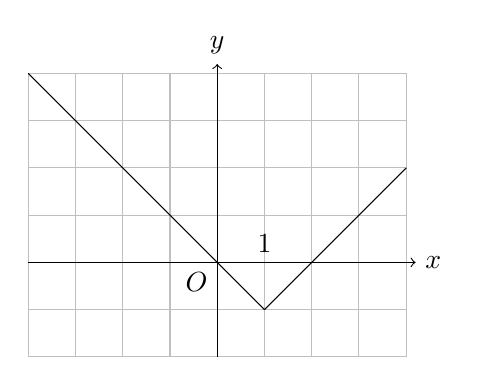
\begin{tikzpicture}[scale=0.6]
		\draw[thin,color=gray!50] (-4,-2) grid (4,4);
		\draw[->] (-4,0) -- (4.2,0) node[right] {$x$};
		\draw[->] (0,-2) -- (0,4.2) node[above] {$y$};
		\draw[domain=-4:1] plot (\x,-\x);
		\draw[domain=1:4] plot (\x,\x-2);
		\draw (0,0) node[below left]{$O$};
		\draw (1,0) node[above]{$1$};
		\end{tikzpicture}}
	{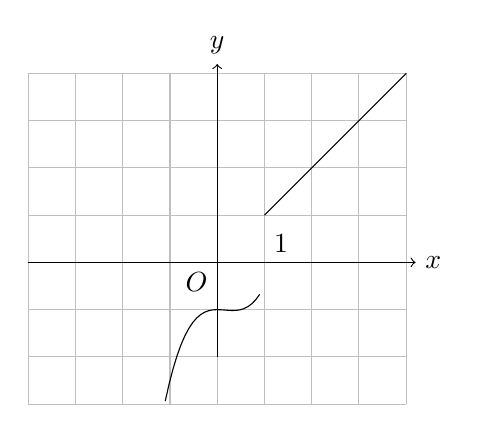
\begin{tikzpicture}[scale=0.6]
		\draw[thin,color=gray!50] (-4,-3) grid (4,4);
		\draw[->] (-4,0) -- (4.2,0) node[right] {$x$};
		\draw[->] (0,-2) -- (0,4.2) node[above] {$y$};
		\draw[domain=-1.1:0.9] plot (\x,{(\x)^3-0.5*(\x)^2-1});
		\draw[domain=1:4] plot (\x,\x);
		\draw (0,0) node[below left]{$O$};
		\draw (1,0) node[above right]{$1$};
		\end{tikzpicture}}
	{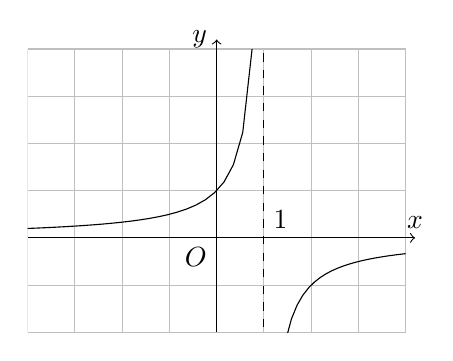
\begin{tikzpicture}[scale=0.6]
		\clip (-4,-2) rectangle (4.4,4.45);
		\draw[thin,color=gray!50] (-4,-2) grid (4,4);
		\draw[->] (-4,0) -- (4.2,0) node[above] {$x$};
		\draw[->] (0,-2) -- (0,4.2) node[left] {$y$};
		\draw[domain=-4:0.75] plot (\x,{(-1)/((\x)-1)});
		\draw[domain=1.1:4] plot (\x,{(-1)/((\x)-1)});
		\draw [dashed] (1,-4)--(1,4);
		\draw (0,0) node[below left]{$O$};
		\draw (1,0) node[above right]{$1$};
		\end{tikzpicture}}
	{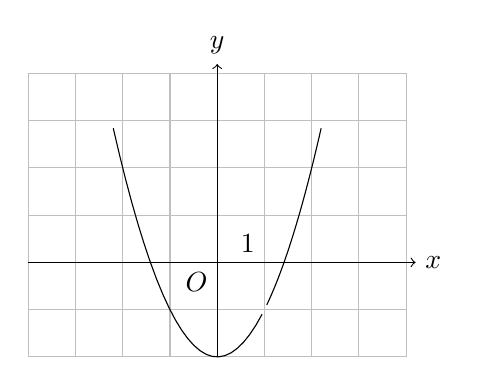
\begin{tikzpicture}[scale=0.6]
		\draw[thin,color=gray!50] (-4,-2) grid (4,4);
		\draw[->] (-4,0) -- (4.2,0) node[right] {$x$};
		\draw[->] (0,-2) -- (0,4.2) node[above] {$y$};
		\draw[domain=-2.2:0.95] plot (\x,{(\x)^2-2});
		\draw[domain=1.05:2.2] plot (\x,{(\x)^2-2});
		\draw (0,0) node[below left]{$O$};
		\draw (1,0) node[above left]{$1$};
		\end{tikzpicture}}
	\loigiai{
		Hàm số có đồ thị như sau liên tục tại $x_0=1$.
		\begin{center}
			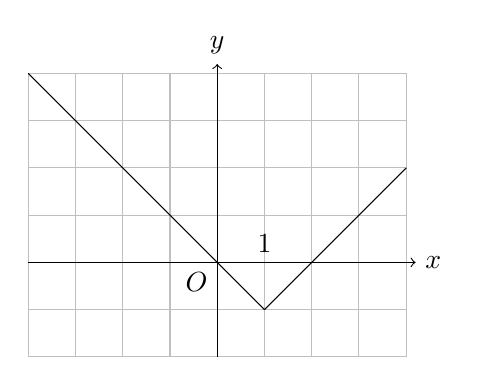
\begin{tikzpicture}[scale=0.6]
			\draw[thin,color=gray!50] (-4,-2) grid (4,4);
			\draw[->] (-4,0) -- (4.2,0) node[right] {$x$};
			\draw[->] (0,-2) -- (0,4.2) node[above] {$y$};
			\draw[domain=-4:1] plot (\x,-\x);
			\draw[domain=1:4] plot (\x,\x-2);
			\draw (0,0) node[below left]{$O$};
			\draw (1,0) node[above]{$1$};
			\end{tikzpicture}
		\end{center}
	}
\end{ex}	
\begin{ex}%[1D3N3-1]%[Dự án đề cương 3 khối năm học 2024 - 2025]%[LamNguyen]
	Cho hàm số $y=f( x )$ liên tục trên $(a;b)$. Điều kiện cần và đủ để hàm số liên tục trên $\left[a;b \right]$ là
	\choice
	{$\lim\limits_{x\to a^+}f(x)=f(a)$ và $\underset{x\to b^+}{\mathop{\lim }}\,f(x)=f(b)$}
	{\True $\lim\limits_{x\to a^+}f(x)=f(a)$ và $\lim\limits_{x\to b^-}f(x)=f(b)$}
	{$\lim\limits_{x\to a^-}f(x)=f(a)$ và $\lim\limits_{x\to b^+}f(x)=f(b)$}
	{$\lim\limits_{x\to a^-}f(x)=f(a)$ và $\lim\limits_{x\to b^-}f(x)=f(b)$}
	\loigiai{
		Hàm số $y=f( x )$ liên tục trên $(a;b)$.\\
		Điều kiện cần và đủ để hàm số liên tục trên $\left[ a;b \right]$ là $\lim\limits_{x\to a^+}f(x)=f(a)$ và $\lim\limits_{x\to b^-}f(x)=f(b)$.
	}
\end{ex}
\begin{ex}%[Dự án đề cương 3 khối năm học 2024 - 2025]%[LamNguyen]%[1D3H3-3]
	Cho $f(x)$, $g(x)$ là các hàm số liên tục tại $x=3$. Biết $f(3)=4$ và $\lim\limits_{x\to 3}\left[ 3f(x)-g(x) \right]=6$. Tính $g(3)$.
	\choice
	{\True $g(3)=6$}
	{$g(3)=0$}
	{$g(3)=2$}
	{$g(3)=-6$}
	\loigiai{
		Vì $f(x)$, $g(x)$ là các hàm số liên tục tại $x=3$ nên
		\begin{eqnarray*}
			&&\lim\limits_{x\to 3}\left[ 3f( x )-g( x ) \right]=6 \\ &\Leftrightarrow& 3\lim\limits_{x\to 3}f( x )-\lim\limits_{x\to 3}g( x )=6\\
			& \Leftrightarrow& 3\cdot 4-\lim\limits_{x\to 3}g( x )=6\\
			& \Leftrightarrow& \lim\limits_{x\to 3}g( x )=6 
		\end{eqnarray*}
		Suy ra $g(3)=6$.		
	}
\end{ex}
\begin{ex}%[Dự án đề cương 3 khối năm học 2024 - 2025]%[LamNguyen]%[1D3N3-4]
	Hàm số nào sau đây \textbf{không} liên tục trên tập số thực $\mathbb{R}$?
	\choice
	{\True $y=\dfrac{4}{x}+\dfrac{7}{9}$}
	{$y=4x+\dfrac{7}{9}$}
	{$y=\sin2x$}
	{$y=3x^2+\sqrt{5}$}
	\loigiai{
		Hàm số $y=\dfrac{4}{x}+\dfrac{7}{9}$ có tập xác định là $\mathbb{R}\setminus \left\{ 0 \right\}$.\\
	 Vì hàm số không xác định tại $0$ nên hàm số không liên tục tại $0$ tức là hàm số đã cho không liên tục trên $\mathbb{R}$.
	}
\end{ex}
\begin{ex}%[Dự án đề cương 3 khối năm học 2024 - 2025]%[LamNguyen]%[1D3N3-3]
	Hàm số nào sau đây \textbf{không} liên tục tại $x=2$?
	\choice
	{$y=\sin x$}
	{\True $y=\dfrac{x^2}{x-2}$}
	{$y=x^2-3x+2$}
	{$y=\sqrt{x+2}$}
	\loigiai{
		Ta thấy hàm số $y=\dfrac{x^2}{x-2}$ có tập xác định là $\mathscr{D}=\mathbb{R}\backslash \left\{ 2 \right\}$ nên hàm số không liên tục tại $x=2$.}
\end{ex}
\begin{ex}%[Dự án đề cương 3 khối năm học 2024 - 2025]%[LamNguyen]%[1D3N3-3]
	Hàm số $f(x)= \heva{&x^2+2 x+m  &\text{ khi } x \geq 2 \\ &3 &\text{ khi } x<2}$ liên tục tại $x=2$ khi
	\choice
	{$m=3$}
	{$m=5$}
	{$m=-3$}
	{\True $m=-5$}
	\loigiai{
		Tập xác định $\mathscr{D}=\mathbb{R}$.\\
		Hàm số liên tục tại $x=2 \Leftrightarrow \lim\limits_{x \to 2^-}f(x)=\lim\limits_{x\to 2^+} f(x)=f(2)\Leftrightarrow 8+m=3\Leftrightarrow m=-5$.
	}
\end{ex}
\begin{ex}%[Dự án đề cương 3 khối năm học 2024 - 2025]%[LamNguyen]%[1D3H3-4]
	Cho bốn hàm số $f_1(x)=2x^3-3x+1$, $f_2(x)=\dfrac{3x+1}{x-2}$, $f_3(x)=\cos x+3$ và $f_4(x)=\tan x$. Hỏi có bao nhiêu hàm số liên tục trên tập $\mathbb{R}$?
	\choice
	{$1$}
	{\True $2$}
	{$3$}
	{$4$}
	\loigiai{
		\begin{itemize}
			\item  Ta có hai hàm số $f_2(x)=\dfrac{3x+1}{x-2}$ và $f_4(x)=\tan x$ có tập xác định không phải là tập $\mathbb{R}$ nên không liên tục trên tập $\mathbb{R}$.
			\item Cả hai hàm số $f_1(x)=2x^3-3x+1$ và $f_3(x)=\cos x+3$ đều có tập xác định là $\mathbb{R}$ và là hàm sơ cấp nên liên tục trên $\mathbb{R}$.
		\end{itemize}
	}
\end{ex}

\begin{ex}%[1D3N3-4]%[Dự án đề cương 3 khối năm học 2024 - 2025]%[LamNguyen]
	Trong các hàm số sau, hàm số nào liên tục trên $\mathbb{R}$?
	\choice
	{$y = \tan x$}
	{$y = \sqrt{2025 + x}$}
	{$y = \dfrac{x + 1}{x - 3}$}
	{\True $y = x^3 + 2x^2 - 4$}
	\loigiai{Hàm số $y = x^3 + 2x^2 - 4$ là hàm đa thức có tập xác định $\mathscr{D}=\mathbb{R}$ nên liên tục trên $\mathbb{R}$.
	}
\end{ex}

\begin{ex}%[LamNguyen]%[1D3N3-3]%[Dự án đề cương 3 khối năm học 2024 - 2025]
	Hàm số $y=\dfrac{1}{x(x^2-9)}$ liên tục tại điểm nào dưới đây?
	\choice
	{$0$}
	{$3$}
	{$-3$}
	{\True $1$}
	\loigiai{
		Điều kiện xác định: $x(x^2-9)\ne 0\Leftrightarrow \heva{& x\ne 0 \\& x\ne \pm 3}$. Vậy tập xác định của hàm số là $\mathscr{D}= ( -\infty;-3 ) \cup ( -3;0 )\cup ( 0;3 ) \cup ( 3;+\infty  )$.\\
		Suy ra hàm số liên tục trên các khoảng $( -\infty;-3 )$, $( -3;0 )$, $( 0;3 )$, $( 3;+\infty  )$.\\
		Ta có $1 \in ( 0;3 )$, vậy hàm số liên tục tại $x=1$.	
	}
\end{ex}
\begin{ex}%[1D3N3-3]%[Dự án đề cương 3 khối năm học 2024 - 2025]%[LamNguyen]
	Hàm số $y=\dfrac{1}{4x-4}$ gián đoạn tại điểm nào dưới đây?
	\choice
	{\True $x=1$}
	{$x=0$}
	{$x=2$}
	{$x=-1$}
	\loigiai{
		Tập xác định $\mathscr{D}=\mathbb{R}\backslash \left\{ 1 \right\}$, suy ra hàm số gián đoạn tại $x=1$.	
	}
\end{ex}



\begin{ex}%[1D3N3-4]%[Dự án đề cương 3 khối năm học 2024 - 2025]%[LamNguyen]
	Hàm số nào sau đây liên tục trên $\mathbb{R}$?
	\choice
	{$y=\cot x$}
	{$y= \tan x$}
	{\True $y=3x^2+2x$}
	{$y=\sqrt{x}$}
	\loigiai{
		Hàm số đa thức liên lục trên toàn bộ tập số thực $\mathbb{R}$.
	}
\end{ex}
\begin{ex}%[1D3H3-3]%[Dự án đề cương 3 khối năm học 2024 - 2025]%[LamNguyen]
	Cho hàm số $f(x)=\heva{
		& \dfrac{x^3+8}{4x+8}\; &\text{ khi } x\ne -2 \\ 
		& 3\; &\text{ khi } x=-2}$. Chọn khẳng định đúng trong các khẳng định sau.
	\choice
	{Hàm số $f( x )$ không liên tục trên tập $\mathbb{R}$}
	{Hàm số $f( x )$ có tập xác định là $\mathbb{R}\setminus \left\{ -2 \right\}$}
	{Hàm số $f( x )$ gián đoạn tại $x=2$}
	{\True Hàm số $f( x )$ liên tục tại $x=-2$}
	\loigiai{
		Tập xác định: $\mathscr{D}=\mathbb{R}$.\\
		Ta có $f(-2)=3$ và \\
		$\lim\limits_{x\to -2}f(x)=\lim\limits_{x\to -2}\dfrac{x^3+8}{4x+8}=\lim\limits_{x\to -2}\dfrac{(x+2)(x^2-2x+4)}{4( x+2 )}=\lim\limits_{x\to -2}\dfrac{x^2-2x+4}{4}=3$.\\
		Suy ra $\lim\limits_{x\to -2}f( x )=f( -2 )$ hay hàm số $f( x )$ liên tục tại $x=-2$.}
\end{ex}
\begin{ex}%[1D3H3-3]%[Dự án đề cương 3 khối năm học 2024 - 2025]%[LamNguyen]
	Cho hàm số $f(x)=\heva{&\dfrac{x^2-3x+2}{x-1}&\quad& \text{khi} \quad x\neq 1\\&a &\quad& \text{khi} \quad  x=1}$. Xác định các giá trị của tham số $a$ để hàm số $y=f(x)$ liên tục tại điểm $x=1$.
	\choice
	{$a=-\dfrac{1}{2}$}
	{\True $a=-1$}
	{$a=0$}
	{$a=\dfrac{1}{2}$}
	\loigiai{
		Tập xác định của hàm số là $\mathrm{D}=\mathbb{R}$.\\
		\begin{itemize}
			\item
			Ta có $\lim\limits_{x\to 1}f(x)=\lim\limits_{x\to 1}\dfrac{x^2-3x+2}{x-1}=\lim\limits_{x\to 1}\dfrac{(x-1)(x-2)}{x-1}=\lim\limits_{x\to 1}(x-2)=-1$.
			\item $f(1)=a$.
		\end{itemize}
		Hàm số $y=f(x)$ liên tục tại điểm $x=1$ khi và chỉ khi $\lim\limits_{x\to 1}f(x)=f(1) \Leftrightarrow a=-1$.
	}
\end{ex}
\Closesolutionfile{ans}

\ind{PHẦN II.} \inden{Câu trắc nghiệm đúng sai. Trong mỗi ý a), b), c), d) ở mỗi câu, học sinh chọn đúng hoặc sai.}\\
\setcounter{ex}{0}
\Opensolutionfile{ans}[ans/2D1-Bai1-DS]%--Đặt tên 2D1-Bai1-DS
\begin{ex}%Câu 2%[1D3H3-3]
	Cho hàm số $f(x)=\heva{& \dfrac{x^2-1}{x-1}&\text{ khi }\,x\ne 1 \\ 
		& x+1&\text{ khi }\,x=1.}$ và $g(x)=4x^2-x+1$. Khi đó
	\choiceTF
	{\True $f(1)=2$}
	{\True Hàm số $f(x)$ liên tục tại điểm $x_0=1$}
	{\True Hàm số $g(x)$ liên tục tại điểm $x_0=1$}
	{Hàm số $y=f(x)-g(x)$ không liên tục tại điểm $x_0=1$}
	\loigiai{
		\begin{itemchoice}
			\itemch \textbf{Đúng.} $f(x_0)=f(1)=1+1=2$.
			\itemch \textbf{Đúng.} $\lim\limits_{x\to x_0} f(x)=\lim\limits_{x\to 1} \dfrac{x^2-1}{x-1}=\lim\limits_{x\to 1}(x+1)=2=f(x_0)$.\\
			Vậy hàm số liên tục tại điểm $x_0=1$.
			\itemch \textbf{Đúng.} Ta có $g(x_0)=g(1)=4$.
			$\lim\limits_{x\to 1}g(x)=\lim\limits_{x\to 1}( 4x^2-x+1)=4=g(1)$.\\
			Vậy hàm số liên tục tại điểm $x_0=1$.	
			\itemch \textbf{Sai.} Vì hai hàm số $f(x)$ và $g(x)$ đều liên tục $x_0=1$ nên hàm số $y=f(x)-g(x)$ liên tục tại điểm $x_0=1$.
		\end{itemchoice}
	}	
\end{ex}
\begin{ex}[\itshape{Đề kiểm tra Toán 11 HKI NH23-24 - THPT Phan Bội Châu}]%[1D3H3-4]%[Dự án đề cương 3 khối năm học 2024 - 2025]%[LamNguyen]
	Cho hai hàm số $f(x)=x-1$ và $g(x)=x^2-3x+2$.	
	\choiceTF
	{\True Hàm số $g(x)$ liên tục trên $\mathbb{R}$}
	{\True Hàm số $y=f(x)+g(x)$ liên tục trên $\mathbb{R}$}
	{Hàm số $y=\dfrac{f(x)}{g(x)}$ liên tục trên $\mathbb{R}$}
	{\True Hàm số $y=\dfrac{g(x)}{f(x)}$ liên tục trên các khoảng $(-\infty;1)$ và $(1;+\infty)$}
	\loigiai{
		\begin{itemchoice}
			\itemch \textbf{Đúng.} Hàm số $g(x)=x^2-3x+2$ có tập xác định là $\mathbb{R}$ nên liên tục trên $\mathbb{R}$.
			\itemch	\textbf{Đúng.} Hàm số $y=f(x)+g(x)=x^2-2x+1$  có tập xác định là $\mathbb{R}$ nên liên tục trên $\mathbb{R}$.
			\itemch	\textbf{Sai.} Ta có $y=\dfrac{f(x)}{g(x)}=\dfrac{x-1}{x^2-3x+2}$.\\
			Hàm số $y=\dfrac{f(x)}{g(x)}$ xác định $\Leftrightarrow x^2-3x+2 \neq 0 \Leftrightarrow \heva{&x \neq 1\\&x \neq 2.}$\\
			Vậy tập xác định của hàm số $y=\dfrac{f(x)}{g(x)}$ là $\mathscr{D}=\mathbb{R} \setminus \left\{1;2\right\}$ nên hàm số $y=\dfrac{f(x)}{g(x)}$ không liên tục trên $\mathbb{R}$.
			\itemch \textbf{Đúng.} Ta có $y=\dfrac{g(x)}{f(x)}=\dfrac{x^2-3x+2}{x-1}$.\\
			Hàm số $y=\dfrac{g(x)}{f(x)}$ xác định $\Leftrightarrow x-1 \neq 0 \Leftrightarrow x \neq 1$.\\
			Vậy tập xác định của hàm số $y=\dfrac{g(x)}{f(x)}$ là $\mathscr{D}=\mathbb{R} \setminus \left\{1\right\}=(-\infty;1) \cup (1;+\infty)$.\\
			Do đó hàm số $y=\dfrac{g(x)}{f(x)}$ liên tục trên các khoảng $(-\infty;1)$ và $(1;+\infty)$. 
		\end{itemchoice}		
	}
\end{ex}


\begin{ex}[\itshape{Đề kiểm tra Toán 11 HKI NH24-25 - THPT - Nguyễn Quốc Trinh - Hà Nội}]%[1D3H3-3]%[Dự án đề cương 3 khối năm học 2024 - 2025]%[LamNguyen]
	Cho hàm số $f(x)=\heva{&\dfrac{1}{4} x+\dfrac{1}{4} &\text{khi } x \leq 2\\&\dfrac{\sqrt{3x-2}-2}{x-2} &\text{khi } x > 2.}$
	\choiceTF
	{$\lim\limits_{x \to 2^{+}} f(x)=\dfrac{1}{2}$}
	{\True $\lim\limits_{x \to 0} f(x)=\dfrac{1}{4}$}
	{\True Hàm số $f(x)$ liên tục tại $x=2$}
	{\True $\lim\limits_{x \to 2^{-}} f(x)=\dfrac{3}{4}$}
	\loigiai{
		\begin{itemchoice}
			\itemch \textbf{Sai}. Ta có 
			\allowdisplaybreaks
			\begin{eqnarray*}
				\lim\limits_{x \to 2^{+}} f(x)&=&\lim\limits_{x \to 2^{+}}\dfrac{\sqrt{3x-2}-2}{x-2}
				\\
				&=&\lim\limits_{x \to 2^{+}}\dfrac{3x-2-4}{(x-2)\left(\sqrt{3x-2}+2\right)}
				\\
				&=&\lim\limits_{x \to 2^{+}}\dfrac{3(x-2)}{(x-2)\left(\sqrt{3x-2}+2\right)}
				\\
				&=&\lim\limits_{x \to 2^{+}}\dfrac{3}{\sqrt{3x-2}+2}
				\\
				&=&\dfrac{3}{4}.			
			\end{eqnarray*}
			\itemch \textbf{Đúng}. Ta có $\lim\limits_{x \to 0} f(x)=\lim\limits_{x \to 0}\left(\dfrac{1}{4} x+\dfrac{1}{4}\right)=\dfrac{1}{4}$.
			\itemch \textbf{Đúng}. Ta có $f(2)=\dfrac{1}{4}\cdot 2+\dfrac{1}{4}=\dfrac{3}{4}$.\\
			Ta có $\lim\limits_{x \to 2^{-}} f(x)=\lim\limits_{x \to 2^{-}}\left(\dfrac{1}{4} x+\dfrac{1}{4}\right)=\dfrac{3}{4}$.\\
			Suy ra $\lim\limits_{x \to 2^{-}} f(x)=\lim\limits_{x \to 2^{+}} f(x)=f(2)$.\\
			Do đó $f(x)$ liên tục tại $x=2$.
			\itemch \textbf{Đúng}. Ta có $\lim\limits_{x \to 2^{-}} f(x)=\lim\limits_{x \to 2^{-}}\left(\dfrac{1}{4} x+\dfrac{1}{4}\right)=\dfrac{3}{4}$.
		\end{itemchoice}
	}
\end{ex}

\begin{ex}[\itshape{Đề kiểm tra Toán 11 HKI NH24-25 - THPT Nguyễn Thái Bình - Tp HCM}]%[1D3H3-3]%[Dự án đề cương 3 khối năm học 2024 - 2025]%[LamNguyen]
	Cho hàm số $f(x)=\left\{\begin{array}{ll}\dfrac{\sqrt{x+3}-2}{x-1} & \text{khi}\,x>1 \\ -x^2+m &  \text{khi}\,x \leq 1\end{array}\right.$. Các mệnh đề sau đây đúng hay sai?
	\choiceTF
	{\True Hàm số xác định trên $\mathbb{R}$}
	{\True $f(1)=-1+m$}
	{$\displaystyle\lim\limits_{x \rightarrow 1^{-}}f(x)=1+m$}
	{Hàm số liên tục tại $x=1$ khi $m=-\dfrac{3}{4}$}
	\loigiai{
		\begin{itemchoice}
			\itemch \textbf{Đúng}.
			Khi $x>1$ thì hàm số là $y=f(x)=\dfrac{\sqrt{x+3}-2}{x-1}$ xác định với mọi $x>1$.\\
			Khi $x \leq 1$ thì hàm số là $y=f(x)=-x^2+m$ xác định với mọi $x\le 1$.\\
			Do đó tập xác định của hàm số $y=f(x)$ là $\mathscr{D}=\mathbb{R}$.
			\itemch \textbf{Đúng}.
			Ta có $f(1)=-(1)^2+m=-1+m$.
			\itemch \textbf{Sai}.
			Ta có $\displaystyle\lim\limits_{x \rightarrow 1^{-}}f(x)=\displaystyle\lim\limits_{x \rightarrow 1^{-}}(-x^2+m)=-(1)^2+m=-1+m$.
			\itemch	\textbf{Sai}.
			$\displaystyle\lim\limits_{x \rightarrow 1^{+}}f(x)=\displaystyle\lim\limits_{x \rightarrow 1^{+}}\dfrac{\sqrt{x+3}-2}{x-1}=\displaystyle\lim\limits_{x \rightarrow 1^{+}}\dfrac{x-1}{(x-1)(\sqrt{x+3}+2)}=\displaystyle\lim\limits_{x \rightarrow 1^{+}}\dfrac{1}{\sqrt{x+3}+2}=\dfrac{1}{4}$.\\
			Để hàm số liên tục tại $x=1$ thì \\
			$$ \displaystyle\lim\limits_{x \rightarrow 1^{+}}f(x)=\displaystyle\lim\limits_{x \rightarrow 1^{-}}f(x)=f(1)\Leftrightarrow -1+m=\dfrac{1}{4}\Leftrightarrow m=\dfrac{5}{4}$$.
		\end{itemchoice}
	}
\end{ex}
\begin{ex}%[1D3H3-6]%[Dự án đề cương 3 khối năm học 2024 - 2025]%[LamNguyen]
	Một bãi đậu xe ô tô đưa ra giá $T(x)$ (đồng) khi thời gian đậu xe là $x$ (giờ) như sau:
	$$T(x)=\heva{
	& 50\,000,\,~ 0<x\le 2\\ 
	& 120\,000, \, ~2<x<4\\ 
	& 35\,000x,\, ~x\ge 4.}$$\\
	Xét tính đúng sai của các khẳng định sau:
	\choiceTF
	{\True $T(2)=50\,000$}
	{$\lim\limits_{x \to 4^+}T(x)=120\,000$}
	{\True Hàm số $T(x)$ không liên tục tại $x=4$}
	{\True Hàm số $T(x)$ liên tục trên $[4;+\infty)$}
\loigiai{
\begin{itemchoice}
	\itemch \textbf{Đúng}. $T(2)=50\,000$
	\itemch \textbf{Sai}. $\lim\limits_{x \to 4^+} T(x)=\lim\limits_{x \to 4^+} (35\,000x)=35\,000\cdot4=140\,000$
	\itemch \textbf{Đúng}. $\lim\limits_{x \to 4^-} T(x)= 120\,000\ne\lim\limits_{x \to 4^+} T(x)$ nên không tồn tại $\lim\limits_{x \to 4} T(x)$ suy ra hàm số $T(x)$ không liên tục tại $x=4$.
	\itemch \textbf{Đúng}. Khi $x>4$, $T(x)=35\,000x$ là hàm đa thức nên liên tục trên $(4;+\infty)$.\\
	Ta lại có $\lim\limits_{x \to 4^+} T(x)=T(4)$ nên hàm số $T(x)$ liên tục trên $[4;+\infty)$.
\end{itemchoice}
}
\end{ex}

\Closesolutionfile{ans}


\ind{PHẦN III.} \inden{Câu trắc trả lời ngắn.}\\
\setcounter{ex}{0}
\Opensolutionfile{ans}[ans/2D1-Bai1-DS]%--Đặt tên 2D1-Bai1-DS
\begin{ex}[\itshape{Đề HKI NH24-25 - Sở GD \& ĐT Bắc Giang}]%[1D3H3-3][Dự án đề cương 3 khối năm học 2024 - 2025]%[LamNguyen]
	Cho hàm số $f(x) = \heva{&\dfrac{x^2-4}{x-2}&\text{\,khi\,} & x \ne 2 \\& 3m & \text{\,khi\,}& x=2}$ với $m$ là tham số. Để hàm số $f(x)$ liên tục tại điểm $x_0 = 2$ thì giá trị của $m$ bằng bao nhiêu? (kết quả làm tròn đến chữ số thập phân thứ hai).
	\par\shortans[oly]{$1{,}33$}
	\loigiai{
		Ta có
		\begin{itemize}
			\item $\lim\limits_{x\to 2} f(x)= \lim\limits_{x\to 2} \dfrac{x^2-4}{x-2}=\lim\limits_{x\to 2} \dfrac{(x-2)(x+2)}{x-2}=\lim\limits_{x\to2}(x+2)=2+2=4$.
			\item $f(2)=3m$.
		\end{itemize}
		Hàm số $f(x)$ liên tục tại điểm $x_0=2$ khi và chỉ khi
			$\lim\limits_{x\to2} f(x)=f(2) \Leftrightarrow
			4 = 3m \Leftrightarrow
			m =\dfrac{4}{3}.$\\
		Vậy $m=\dfrac{4}{3}\approx1{,}33$.
	}
\end{ex}
\begin{ex}%[1D3V3-3]%[Dự án đề cương 3 khối năm học 2024 - 2025]%[LamNguyen]
	Cho hàm số $y=f(x)=\heva{&10&& \text{khi}~0\le x\le 5\\
		&x^2+ax+10&& \text{khi}~ x>5}$. Tìm giá trị của $a$ để hàm số liên tục tại $x_0=5$.
	\shortans[oly]{$-5$}
	\loigiai{Ta có $\heva{&f(5)=10 \\&\lim\limits_{x\to 5^-}f(x)=\lim\limits_{x\to 5^-}10=10 \\& \lim\limits_{x\to 5^+}f(x)=\lim\limits_{x\to 5^+}\left(x^2+ax+10\right)=35+5a.}$\\
		Hàm số đã cho liên tục tại $x_0=5$ khi và chỉ khi $f(5)=\lim\limits_{x\to 5^-}f(x)=\lim\limits_{x\to 5^+}f(x)$.\\
		Khi đó $10=35+5a\Leftrightarrow a=-5$.}
\end{ex}
\begin{ex}[Đề KT - NH 2425 - THPT Phan Bội Châu - Bình Thuận]%[1D3V3-3][Dự án đề cương 3 khối năm học 2024 - 2025]%[LamNguyen]
	Biết hàm số $f(x)=\heva{& \dfrac{x^2+ax+2}{x-1}& \text{ khi } x\ne 1 \\ & b & \text{ khi } x=1}$ liên tục tại $x=1\,\left(a,\,b\in\mathbb{R},~b\ne 0\right)$. Khi đó giá trị $a+b$ bằng bao nhiêu?
	\shortans[oly]{$-4$}
	\loigiai{
		Do hàm số liên tục tại $x=1$ nên 
		$\lim \limits_{x \to 1}f(x)=\lim \limits_{x\to 1}\dfrac{x^2+ax+2}{x-1}=f(1)=b$.\\
		Do $\lim \limits_{x \to 1}\left(x-1\right)=0$ nên để giới hạn hữu hạn $\lim \limits_{x \to 1}\dfrac{x^2+ax+2}{x-1}$ tồn tại thì  $$\lim \limits_{x\to 1}\left(x^2+ax+2\right)=0\Rightarrow a+3=0\Rightarrow a=-3.$$\\
		Khi đó
		\begin{eqnarray*}
			\lim \limits_{x\to 1}f(x)&=&\lim \limits_{x\to 1}\dfrac{x^2+ax+2}{x-1}\\
			&=&\lim \limits_{x\to 1}\dfrac{x^2-3x+2}{x-1}\\
			&=&\lim \limits_{x\to 1}\dfrac{\left(x-1\right)\left(x-2\right)}{x-1}\\
			&=&\lim \limits_{x\to 1}\left(x-2\right)=-1.\\ 
		\end{eqnarray*} 
Suy ra $b=-1$, vậy $a+b=-4.$}
\end{ex}
\begin{ex}[\itshape{Đề HKI - NH24-25 - THPT Nguyễn Thái Bình - Tp HCM }]%[1D3V3-4]%[Dự án đề cương 3 khối năm học 2024 - 2025]%[LamNguyen]
	Tìm giá trị lớn nhất của $a$ để hàm số $f(x)=\heva{&\dfrac{\sqrt[3]{3x+2}-2}{x-2}& \text{ khi } x >2 \\  &a^2 x-\dfrac{1}{4}&\text{  khi } x\le2}$  liên tục tại $x=2$.\\
	\shortans[oly]{$0{,}5$}
	\loigiai{
		Ta có 
		\begin{eqnarray*}
			& & \lim\limits_{x \to 2^+} f(x) =  \lim\limits_{x \to 2^+} \dfrac{\sqrt[3]{3x+2}-2}{x-2}\\
			&= & \lim\limits_{x \to 2^+} \dfrac{3x - 6}{ (x-2) \left[\left(\sqrt[3]{3x+2}\right)^2+\sqrt[3]{3x+2}\cdot2+4\right]}  \\
			&=& \lim\limits_{x \to 2^+} \dfrac{3}{\left(\sqrt[3]{3x+2}\right)^2+\sqrt[3]{3x+2}\cdot2+4}\\
			&=&\dfrac{3}{3 \cdot 4} = \dfrac{1}{4}.
		\end{eqnarray*}
		Mặt khác: $ \lim\limits_{x \to 2^-} f(x) = f(2) = 2a^2 -\dfrac{1}{4}. $\\
		Để hàm số liên tục tại điểm $ x_0 = 2$ thì $$\lim\limits_{x \to 2^+} f(x)=\lim\limits_{x \to 2^-} f(x)  = f(2) \Leftrightarrow 2a^2 -\dfrac{1}{4}=\dfrac{1}{4}\Leftrightarrow a^2=\dfrac{1}{4}\Leftrightarrow \hoac{&a=\dfrac{1}{2}\\&a=\dfrac{-1}{2}}.$$
		Vậy giá trị lớn nhất của $a=\dfrac{1}{2}$.
	}
\end{ex}
\begin{ex}%[1D3H3-6]%[Dự án đề cương 3 khối năm học 2024 - 2025]%[LamNguyen]
	Một chuyển động thẳng biến đổi đều trong 5 giây đầu có phương trình đường đi là $ S(t)=2t^2+10t$ và sau đó tiếp tục chuyển động theo phương trình $S(t)=a{t^2}+3t$ trong đó $S$ tính bằng mét, $t$ tính bằng giây. Tìm giá trị của $a$.
	\shortans[oly]{$3{,}4$}
\loigiai{
	Ta có phương trình của chuyển động là $S(t)=\heva{
	& 2t^2+10t\,~\text{khi}~\,0\le t\le 5\\ 
	& a{t^2}+3t\,~\text{khi}~\,t>5.}$\\
	Dễ thấy phương trình chuyển động $S(t)$ là hàm số liên tục.\\
	Hàm số $ S(t)$ liên tục trên các khoảng $\left(0;\,5\right)$ và $\left(5;\,+\infty\right)$ để hàm số $ S(t)$ liên tục thì nó phải liên tục tại $ t=5$.\\
	Ta có $\lim\limits_{t\to 5^-} S(t)=\lim\limits_{t\to 5^-}\left(2t^2+10t\right)=100$;$\lim\limits_{t\to 5^+} S(t)=\lim\limits_{t\to 5^+} \left(a{t^2}+3t\right)=25a+15$; $S(5)=100$.\\
	Hàm số liên tục tại $ t=5$ khi $\lim\limits_{t\to 5^-} S(t)=\lim\limits_{t\to 5^+} S(t)=100\Leftrightarrow 25a+15=100\Leftrightarrow a=\dfrac{17}{5}=3{,}4$.\\
	Vậy $a=3{,}4$.}
\end{ex}
\Closesolutionfile{ans}


\ind{PHẦN IV.} \inden{Tự luận.}\\
\setcounter{ex}{0}
\begin{ex}%[1D3N3-3]%[Dự án đề cương 3 khối năm học 2024 - 2025]%[LamNguyen]
	Xét tính liên tục của hàm số $f(x)=\dfrac{2}{x-1}$ tại điểm $x_0=2$.
	\loigiai{
		Tập xác định $\mathscr{D}=\mathbb{R}\setminus\{1\}$.\\
		Ta có
		$f(2)=\dfrac{2}{2-1}=2$,
		$\lim\limits_{x \to 2} f(x)= \lim\limits_{x \to 2} \dfrac{2}{x-1} =2$.\\
		Suy ra $\lim\limits_{x \to 2} f(x)=f(2)=2$.\\
		Vậy hàm số liên tục tại $x_0=2$.
	}
\end{ex}

\begin{ex}%[1D3N3-3]%[Dự án đề cương 3 khối năm học 2024 - 2025]%[LamNguyen]
	Cho hàm số  $f(x)=\heva{&x^2+1 & \text{khi }\, x>0&\\ &x & \text{khi }\, x\le 0& }$. Xét tính liên tục của hàm số tại điểm $x_0=0$.
	\loigiai{
		Tập xác định $\mathscr{D}=\mathbb{R}$.\\
		Ta có
		$f(0)=0$.\\
		$\heva{
			&\lim\limits_{x \to 0^+} f(x)= \lim\limits_{x \to 0} (x^2+1) =1\\
			&\lim\limits_{x \to 0^-} f(x)= \lim\limits_{x \to 0} x =0}$
		$\Rightarrow\lim\limits_{x \to 0^+} f(x)\ne \lim\limits_{x \to 0^-} f(x)$.\\
		Do đó không tồn tại $\lim\limits_{x \to 0} f(x)$.\\
		Vậy hàm số $f(x)$ không liên tục (gián đoạn) tại $x_0=0$.
	}
\end{ex}
\begin{ex}[\itshape{ĐỀ KSCL CUỐI HK1 - THPT BẮC YÊN THÀNH - NGHỆ AN}]%[1D3H3-3]%[Dự án đề cương 3 khối năm học 2024 - 2025]%[LamNguyen]
	Tìm giá trị của tham số $m$ để hàm số $f(x)=\heva{&
		\dfrac{x^2-x-2}{x-2} &, \text { khi } x \neq 2 \\
		&m+1 &, \text { khi } x=2
	}$ liên tục tại điểm $x_0=2$.
	\loigiai{
		Ta có $f(2)=m+1$ và $\displaystyle\lim\limits _{x \rightarrow 2}f(x)=\displaystyle\lim\limits _{x \rightarrow 2} \dfrac{x^2-x-2}{x-2}=\displaystyle\lim\limits _{x \rightarrow 2} \dfrac{(x-2)(x+1)}{x-2}=\displaystyle\lim\limits _{x \rightarrow 2} (x+1)=3$.\\
		Để hàm số liên tục tại điểm $x_0=2$ thì $\displaystyle\lim\limits _{x \rightarrow 2} f(x)=f(2) \Leftrightarrow m+1=3 \Leftrightarrow m=2$.
		
	}
\end{ex}
\begin{ex}%[1D3H3-3]%[Dự án đề cương 3 khối năm học 2024 - 2025]%[LamNguyen]
	Xét tính liên tục của hàm số 
	$$ f(x) = \heva{&\dfrac{\sqrt{x + 10} - 3}{x + 1} & \text{khi } x > -1 \\ &\dfrac{x + 2}{5 - x} & \text{khi } x \le -1}$$
	tại điểm $x_0 = -1$.
	\loigiai{
		$\bullet$ Ta có 
		\allowdisplaybreaks
		\begin{eqnarray*}
			\lim\limits_{x \to (-1)^+} f(x) &=& \lim\limits_{x \to (-1)^+} \dfrac{\sqrt{x+10}-3}{x+1} \\
			&=& \lim\limits_{x \to (-1)^+}\dfrac{x+10-3^2}{(x+1)\left(\sqrt{x+10}+3\right)} \\
			&=& \lim\limits_{x \to (-1)^+}\dfrac{x+1}{(x+1)\left(\sqrt{x+10}+3\right)} \\ &=&\lim\limits_{x \to (-1)^+} \dfrac{1}{\sqrt{x+10}+3} \\
			&=& \lim\limits_{x \to (-1)^+} \dfrac{1}{\sqrt{-1+10}+3} \\
			&=& \dfrac{1}{6}.
		\end{eqnarray*}
		$\bullet$ $\lim\limits_{x \to (-1)^-} f(x) = \lim\limits_{x \to (-1)^-} \dfrac{x+2}{5-x} = \dfrac{-1+2}{5-(-1)} = \dfrac{1}{6}$ và $f(-1) = \dfrac{1}{6}$. \\
		Suy ra $\lim\limits_{x \to (-1)^+} f(x) = \lim\limits_{x \to (-1)^-} f(x) = f(-1)$. \\
		Vậy hàm số $f(x)$ liên tục tại điểm $x_0=-1$.
	}
\end{ex}


\begin{ex}%[1D3H3-4]%[Dự án đề cương 3 khối năm học 2024 - 2025]%[LamNguyen]
	Xét tính liên tục của hàm số $f(x)= \heva{&\sqrt{x+4} & \text { khi } x \geq 0 \\ &2 \cos x & \text { khi } x<0.}$
	\loigiai{
		\begin{itemize}
			\item[$\bullet$] Khi $x>0$: $f(x)=\sqrt{x+4}$ liên tục.
			\item[$\bullet$] Khi $x<0$: $f(x)=2\cos x$ liên tục.
			\item[$\bullet$] Tại $x=0$: $\lim\limits_{x\to 0^+} f(x)=\lim\limits_{x\to 0^-} f(x)=f(0)=2$ $\Rightarrow$ hàm số $y=f(x)$ liên tục tại $x=0$.
		\end{itemize}
		Vậy hàm số $y=f(x)$ liên tục trên $\mathbb{R}$.
	}	
\end{ex}
\begin{ex}%[1D3H3-4]%[Dự án đề cương 3 khối năm học 2024 - 2025]%[LamNguyen]
	Cho hàm số $f(x)=2x-\sin x$, $g(x)=\sqrt{x-1}$.\\ 
	Xét tính liên tục của hàm số $y=f(x)\cdot g(x)$ và $y=\dfrac{f(x)}{g(x)}$.
	\loigiai{\begin{itemize}
			\item Hàm số $f(x)=2x-\sin x$ liên tục tại mọi điểm $x_0\in\mathbb{R}$.
			\item Hàm số $g(x)=\sqrt{x-1}$ liên tục tại mọi điểm $x_0\ge1$.
			\item Ta có $g(x)=0\Leftrightarrow x-1=0\Leftrightarrow x=1$.
		\end{itemize}
		Vậy ta có hàm số $y=f(x)\cdot g(x)$ liên tục tại mọi điểm $x_0\ge1$, hàm số $y=\dfrac{f(x)}{g(x)}$ liên tục tại mọi điểm $x_0>1$.}
\end{ex}
\begin{ex}%[1D3H3-5]%[Dự án đề cương 3 khối năm học 2024 - 2025]%[LamNguyen]
	Chứng minh rằng phương trình $x+1+\cos x=0$  có nghiệm.
	\loigiai{
		Xét hàm số $f(x)=x+1+\cos x$ liên tục trên $\left[-\pi ;0\right]$ và có $\heva{
			& f\left(-\pi \right)=-\pi  \\ 
			& f(0)=2 \\
		}\Rightarrow f\left(-\pi \right)\cdot f(0)<0$. \\
	Suy ra phương trình $f(x)=0$ có nghiệm $x_0\in \left(-\pi ;0\right)$.\\
		Vậy phương trình $x+1+\cos x=0$  có nghiệm.	
	}
\end{ex}
\begin{ex}%[1D3H3-5]%[Dự án đề cương 3 khối năm học 2024 - 2025]%[LamNguyen] 
	Chứng minh rằng phương trình $x^5-3x-7=0$ có ít nhất một nghiệm.
	\loigiai{
		Xét hàm số $f(x)=x^5-3x-7$ là hàm đa thức liên tục trên $\mathbb{R}$ nên nó liên tục trên $[0;2]$.\\
		Ta có $f( 0 )=-7$, $f(2)=19$ nên $f(0)\cdot f(2)<0$. Khi đó phương trình $f(x)=0$ có ít nhất một nghiệm trong khoảng $(0;2)$.} 
\end{ex}
\begin{ex}[\itshape{SGK CTST 11}]%[1D3V3-4]
	Trong một phòng thí nghiệm, nhiệt độ trong tủ sấy được điều khiển tăng từ $10^{\circ} \mathrm{C}$, mỗi phút tăng $2^{\circ} \mathrm{C}$ trong $60$ phút, sau đó giảm mỗi phút $3^{\circ} \mathrm{C}$ trong $40$ phút. Hàm số biểu thị nhiệt độ (tính theo $^{\circ} \mathrm{C}$ ) trong tủ theo thời gian $t$ (tính theo phút) có dạng
	$$
	T(t)= \heva{&10+2 t & \text { khi } 0 \leq t \leq 60 \\ &k-3 t & \text { khi } 60<t \leq 100}\ (k \text{ là hằng số}).
	$$
	Biết rằng, $T(t)$ là hàm liên tục trên tập xác định. Tìm giá trị của $k$.
	\loigiai{
		Vì $T(t)$ là hàm liên tục trên tập xác định nên ta có hàm $T(t)$ liên tục tại $t=60$.\\
		Từ đó ta có $\lim\limits_{t\to 60^-} T(t)=\lim\limits_{t\to 60^+} T(t)=T(60)
		\Leftrightarrow 10+2\cdot 60=k-3\cdot 60\Leftrightarrow k=310$.\\
		Vậy $k=310$.
	}
\end{ex}
\begin{ex}%[1D3V3-3]%[Dự án đề cương 3 khối năm học 2024 - 2025]%[LamNguyen]
	Một hãng taxi đưa ra giá cước $T(x)$ (đồng) khi đi quãng đường $x$ (km) cho loại xe $4$ chỗ như sau $T(x)=\heva{
	&10\,000+a\,~\text{khi}~\,0<x\le 0,7\\ 
	&11\,000+15\,100\cdot\left(x-0,7\right)\,~\text{khi}~\,0,7<x\le 30\\ 
	&453\,430+12\,000\cdot\left(x-30\right)\,~\text{khi}\,~x>30.}$\\
Tìm $ a$ để hàm số $T(x)$ liên tục tại $x=0{,}7$.
\loigiai{
	Tại $ x=0,7$ ta có $ T(0{,}7)=10\,000+a$;\\
	 $\lim\limits_{x\to 0{,}7^-} T(x)=\lim\limits_{x\to 0{,}7^-} (10\,000+a)=10\,000+a$.\\
	Ta có $\lim\limits_{x\to 0{,}7^+} T(x)=\lim\limits_{x\to 0{,}7^+} \left[ 11\,000+15\,100\cdot(x-0{,}7)\right] =11\,000$.\\
	Hàm số liên tục tại $x=0{,}7$ thì $\lim\limits_{x\to 0{,}7^-} T(x)=\lim\limits_{x\to 0{,}7^+} T(x)=T(0{,}7)\Leftrightarrow a=1000$.}
\end{ex}
